\chapter{Introduction}\label{introduction}

\settowidth{\epigraphwidth}{Wonderful life : the Burgess Shale and the nature of history}
\epigraph{%
Without hesitation or ambiguity, and fully mindful of such paleontological wonders as large dinosaurs andAfrican ape-men, I state that the invertebrates of the Burgess Shale, found high in the Canadian Rockies in YohoNational Park, on the eastern border of British Columbia, are the world's most important animal fossils. Modern multicellular animals make their first uncontested appearance in the fossil record some 570 million years ago--and with a bang, not a protracted crescendo.}%
{\textit{\\Wonderful life : the Burgess Shale and the nature of history}\\\textsc{Stephen Jay Gould}}

The goal for this work is to determine the conditions under which robust, interesting, adaptive evolution can be started and undergo self-improvement in the non-living world. 

Ongoing evolution means something more than continual change of population frequencies; instead we refer to the goal of a process that continues to produce interesting, novel, and creative results, as does natural biological evolution; in other words, a changing process, and so our goal is the \textit{gls{evoevo}}. Finally, we constrain our domain to software rather than wetware or hardware; simulations and models, rather than elements embedded in the physical world.

Natural evolution is the foundation for several related bodies of literature, in Computational Intelligence and Artificial Life, as well of course of the study of evolution in natural systems. As many have observed, there are major differences between the original inspiration and the spin-offs. Biological evolutionary systems are complex, contingent, emergent, endogenous and general. By contrast, artificial evolutionary systems such as Evolutionary Algorithms are exogenous, problem-specific and designed.

A convenient shorthand capturing these differences labels the biological inspiration as bottoms-up or emergent and the derived fields as top-down or designed. If the top-down approach has failed, then perhaps there might be mileage in returning to biology, our sole example of a general self-improving, self-organizing system.

But as biology is contingent, what is the most useful starting point for a recapitulation? Assume first of all that we are in the domain of software, rather than hardware or wetware, for practical reasons. And also assume that biological evolution does not depend upon embodiment--that the outcome can be adequately modelled at a conceptual level without being grounded in either the physical world, or in contingent biology such as enzymes, proteins and genes.

Then our belief is that the \emph{\gls{evoevo}} itself can and will emerge under certain conditions, and that an emergent approach will be more successful than the predominant design-driven top-down approach today.

%Simple ongoing evolution is not the same as creative or interesting evolution; the current state-of-the-art is both insufficient and unsatisfying. \parencite{Bourrat2015} makes a related distinction between distributive and transformative forms of evolution, where distributive evolution sees simply a change in population distribution without the generation of novelties or new elements characteristic of transformative evolution. The fundamental open problem is how to achieve transformative evolution in artificial systems.

\emph{A copy mechanism with adjustable fidelity can auto-adjust for example to changing environmental conditions.}

\begin{compactitem}
	\item
	      Not same as ENS--that explains natural processes; our goal is to achieve something that is as interesting in a different domain
	\item 
	      Not same as EAs--EAs have exogenous fitness, not open-ended (search through a fixed space, cannot surprise (\eg \parencite{Nellis2014})
	\item  
	      Not same as approach where take ideas from biology and evaluate for different purpose (\eg in EAs, island populations, GRNs (\eg L-systems), Lamarkian learning, co-evolution, evolutionary transitions (cooperation and mediation in \parencite{Defaweux:2005fk}\ldots{}). All seem to follow model of currently we use these tools, biology has something we don't have, let's try it\ldots{}
	\item
	      Not the same as most type of Alife, where evolution is not the subject of the research but rather a tool or mechanism towards some other goal (canonically, creating artificial life.)
\end{compactitem}

Constitutive definitions of \gls{oee}

\parencite{Taylor2001} like others makes a distinction between OEE and ``kinds of evolutionary innovation''. He gives as an example of limited innovation the emergence of paratism in \cite{Ray1991} as direct result of system design and initial seeding conditions. In this reading, ``fundamentally new'' (labelled by Taylor as ``creative'') means new ways of sensing the environment and interacting with it \cite{Taylor2001}.

\quote{by open-ended evolutionary capacity we understand the potential of a system to reproduce its basic functional-constitutive dynamics, bringing about an un-limited variety of equivalent systems, of ways of expressing that dynamics, which are not subject to any predetermined upper bound of organizational complexity (even if they are, indeed, to the energetic-material restrictions imposed by a finite environment and by the universal physico-chemical laws)}{\cite{Ruiz-Mirazo2004}}

\begin{compactitem}
	\item An open-ended evolutionary system must demonstrate unbounded diversity during its growth phase.
	\item An open-ended evolutionary system must embody selection.
	\item An open-ended evolutionary system must exhibit continuing (``positive'') new adaptive activity.
	\item An open-ended evolutionary system must have an endogenous implementation of niches.
\end{compactitem} \cite{Maley1999} (considered ``rather abstract'' by Hutton \parencite[p.341]{Hutton2002}).

``openendedness depends fundamentally on the continual production of novelty.'' Standish, in \parencite{Soros2014}

``we would like the evolutionary system, like life, to continue to produce individuals of increasing complexity and diversity.'' -
although note, following McShea, that much of life is single-celled and hasn't become much more complex in billions of years \parencite{Maley1999}

\quote{by open-ended evolutionary capacity we understand the potential of a system to reproduce its basic functional-constitutive dynamics, bringing about an un-limited variety of equivalent systems, of ways of expressing that dynamics, which are not subject to any predetermined upper bound of organizational complexity (even if they are, indeed, to the energetic-material restrictions imposed by a finite environment and by the universal physico-chemical laws.}{\parencite{Ruiz-Mirazo2004}}

\section{Motivation}

Perpetual production of novelty
unbounded evolution
The potential size and complexity of the individuals' phenotypes should be (in principle) unbounded.  \parencite{Soros2014}
Unlimited heredity--number of possible heritable types should astronomically exceed individuals in population \parencite{Vasas2015}.

continual production of complexity
essence of life

General difficulty with grounding these definitions, as the terms on which they rely are themselves only loosely defined (although commonly understood). \parencite{BanzhafBaumgaertnerBeslonEtAl2016}. As \textcite{Gayon2010} notes, many fundamental things generally taken for granted, such as ``life'' and ``energy'', are hard to define. 

\begin{mdframed}[style=box, frametitle={Creativity, and its relationship to Novelty, Surprise, and Value}]
Creativity is related to exploration--how we explore and what we find--a general problem in Artificial Life, Artificial Evolution, and in fact life in general. That no standard definition exists is a good indication that this is a hard problem. Intuitively, creativity is something that causes a sense of surprise or wonder in an observer. Creative systems and products are beautiful; interesting; impressive; novel; surprising; transformative.  For example, in \parencite{Lehman2012}, creativity is related to beauty and interestingness--while impressiveness is time-independent, interestingness often drops over time.

Following \textcite{Boden2004}, a starting point might be that creativity is a \emph{process} that results in \emph{artifacts} with the properties of novelty, surprise, and value. It's clear that to \cite{Boden2004} not all novelties are creative; creativity means something more than change-for-changes sake. Creativity is the ability to come up with ideas or artifacts that are \begin{inparaenum}[1)]\item new--a jump not just extension,\item surprising--statistically unlikely, or unexpectedly belonging to a class, or thought impossible--a sense of wonder and \item valuable--a sense of a deeper meaning; fitness or appropriateness or usefulness \end{inparaenum}\parencite{Boden2004}. Perkins interprets \cite{Boden2004} as saying that creativity is a search plan that breaks or changes the rules (or representation or landscape) so as to make previously inaccessible (or hard to access or isolated) regions of the search space (the ones that contain new, surprising and valuable items) accessible (or rich) \parencite{Perkins1995}. For example, moving from individual organisms to assemblages or aggregations (changing the level of selection--a rule change) would certainly be seen as novel, surprising and valuable.

For Dorin and Korb \cite{Dorin2009} creativity is primarily connected to rareness--if something was rare but is now less rare in another framework, then the framework is more creative. Value (and incidentally appropriateness) is explicitly denied \cite[p.18]{Dorin2009}, in part because of the difficulty of defining value in a general way. Novelty is important, but comes as a consequence of the introduction of a new framework which generates novel patterns. In \cite[p.16]{Dorin2009} though, novelty is introduced as the time lag between successive more creative frameworks--humans become habituated to ideas, so novelty means surprise. Surprise is therefore equated with one (``unlikely'') of Boden's three ideas of surprising (``unlikely or unfamiliar'', ``unexpectedly belongs to a class'', and ``thought impossible.'')

\emph{Novelty} can be seen as either historical novelty (new to all) or psychological novelty (new to self), where the latter is more interesting as a superset of the former (and removes historical chance.)\footnote{I would argue that in biology, the identification of novelty has been essentially subjective based upon a reading of the historical record to identify patterns and changes in those patterns. Any measures, such as proposed by \cite{McShea1998,Maynard-Smith:1995lw,Walker2012} are post-hoc.}

Almost by definition, novelty is difficult to identify. A straightforward definition would suggest we're interested in changes--identifying significant changes seems reasonable, but changes in what? Pre-identifying characteristics to monitor limits our scope, and our imagination, to those characters. How do we create a list of existing characters as a baseline? How could this be done objectively? And what about completely new characters? How could we ever describe those ahead of time? In other words, if we can describe it ahead of time, it isn't novel. A second related issue is one of \textit{reification}--if these characters emerge from lower-order operations, rather than being specified, then we need a mechanism to identify, capture, and describe each new one.

Systems which are only random are not creative (\eg Racter in \cite[p.16]{Dorin2009})--it seems that novelty is not enough, and random variation within bounds that do not change is quickly seen as normal and not novel. 

Next, changes are obviously relative, so we must identify what we are comparing--within a population there is inherent variation. Do we compare to an average, or to a range? And presumably the population is undergoing evolution, and therefore there will be some underlying trends. To be significant, any change should be more than just an acceleration (or dimunition) of a pre-existing trend. Finally, at what point can we declare a novelty? On its first appearance? Perhaps though the putative novelty is maladaptive, and doesn't last beyond one generation. Perhaps it doesn't even last that long: the individual isn't viable. Hereditary lineages (\eg Fitness Transmission \parencite{Miconi:2007xh}) might be one approach to this. For all of these reasons, any objective measure of novelty based on characters seems in practice impossible. This problem applies to both physical characteristics, such as cellular membranes, or legs, and processes, such as cross-membrane transport or genome replication.

\emph{Surprise} is almost as difficult to define as creativity, as it is also relative in general to an observer, but previous work has successfully equated surprise with rarity (\eg \cite{Kowaliw2009}). Related to surprise, is impressiveness or ``rare and hard-to-recreate'' \parencite{Lehman2012}: an asymmetrical transformation in that is easy to recognize yet hard to create, and so similar to NP-completeness, which can be verified but not solved in polynomial time \parencite{Lehman2012}.

\emph{Valuable} seems at first problematic: valuable to who? Introducing an observer into the definition freights in subjectivity and the associated practical difficulty of capturing the observer's assessments. A pragmatic answer might instead be that it is valuable to itself--valuable ideas are ones that are successful, or in other words, that are of high fitness. 
\footnote{\cite{Bringsjord2000} argues that Boden is wrong in two ways: first, that computer creativity does not shed much insight into human creativity (citing Searle's Chinese Room to demonstrate that shuffling symbols, as a creative AI would do, doesn't add much to our understanding), and second, that Boden's formulation of a rule change is too weak. Systems (citing BRUTUS) that are not considered creative, do rule changes of the form proposed by Boden. Instead, these changes must be more special than simple first-order logic. The first criticism is not relevant to us (echoed by \cite{Dorin2009}), but the second holds.}
\end{mdframed}

\Cite{BanzhafBaumgaertnerBeslonEtAl2016} (an outcome of a workshop held in the summer of 2014 on ``Open-ended Novelty'', attended by many of those whose works are cited elsewhere in this thesis) provide a neat way to formalize novelty by making the idea of \cite{Boden2004}, that novelties ``break the rules'', explicit in the form of models and meta-models. By proposing a standard meta-model to describe any \gls{oee} system, be it living or non-living, \cite{BanzhafBaumgaertnerBeslonEtAl2016} can then define three levels of novelty by their effect on the model of the system itself and the overall meta-model:

\begin{itemize}
	\item Type-0 variation--novelty occurs within the scope of the existing model, by changing the values of existing variables.
	\item Type-1 innovation--changes to the model itself, either new types or relationships.
	\item Type-2 emergence--changes to the meta-model, again either in the form of new meta-types or meta-relationships between meta-types.
\end{itemize}
	
The significance of this formulation is that novelty for almost the first time becomes non-subjective and measurable (assuming agreement on the overall meta-model, and that a model for the specific system can be defined.)

\Textcite{Taylor2001,Taylor:1999sc} discuss creativity in \gls{oee} in depth and argues that, for it to be possible, the replicators must \parencite{Hutton2004}:
\begin{compactenum}
	\item Be fully embedded in their arena of competition 
	\item Have rich, unlimited interactions between each other and with their environment 
	\item Initially replicate implicitly, rather than using some encoding of the replication process, and 
	\item Be constructed entirely of `material' components, allowing the possibility of different encodings of information. (\quote{the very stuff from which they are constructed is a valuable resource of matter and energy}{\cite[s3.6]{Taylor2001}})
\end{compactenum}

``the potential for a large degree of intrinsic adaptation'' \parencite{Taylor2001}

\parencite{Soros2014} presents four necessary conditions for OEE (it is left open if these are also sufficient conditions):
\begin{compactenum}
	\item A rule should be enforced that individuals must meet some minimal criterion (MC) before they can reproduce, and that criterion must be nontrivial.
	\item The evolution of new individuals should create novel opportunities for satisfying the MC
	\item Decisions about how and where individuals interact with the world should be made by the individuals themselves.
	\item The potential size and complexity of the individuals' phenotypes should be (in principle) unbounded.
\end{compactenum}
Along with these specific conditions, \parencite{Soros2014} assumes certain general conditions: a ``good'' genetic representation, a ``sufficiently large world for every individual to be evaluated'', and a seed or starting point.

Minimal conditions for OEE \parencite{Vasas2015}:
\begin{compactenum}
	\item Very rich combinatorial generative mechanism \eg organic chemistry.
	\item Unlimited heredity--number of possible heritable types should astronomically exceed individuals in population (Maynard-Smith:1995lw).
	\item Inexhaustible fitness landscape--implies rich, dynamical environment.
	\item Cannot state in advance possible preadaptations.
\end{compactenum}

Elements/Embodiment/Emergence:
Open-ended evolution can be seen as the outcome of evolution in an open-ended system (\eg Chemistry), where an open-ended system has effectively unrestricted representation: the number of possible types must be much larger than the number of individuals. In the terminology of \cite{Szathmary:2006ty}, these are unlimited replicators, in contrast to limited replicators where the number of possible types is less than the number of individuals. Without this property all possible types can be generated in a finite time, and the system will either reach stasis or begin to repeat. Not all open-ended systems necessarily support evolution, but in those that do, our intuition suggests that open-ended evolution produces increasing complexity, increasing diversity, accumulation of novelty and continual adaptation \parencite{Lehman2012}.

Everything in our artificial world must be built from a common set of raw materials; a loop connects the targets of selection with the environment. Other work, although superficially similar in that it models objects of similar scale, uses different models for the objects and the world (see \parencite{Sanchez-Dehesa:2008uq}) and so lack this loop.

Similar to the \emph{semantic closure} of \cite{Pattee1995a}--``organisms should be constructed `with the parts and laws of an artificial physical world''' \cite{Taylor2001}
Smith-Szathmary hypothesis that major transitions in biology are characterized by new ways of transmitting information. Adami follows this direction in stating ``It is probably more appropriate to say that evolution increases the amount of information a population harbors about its niche (and therefore, its physical complexity).'' \cite{Adami2002}

\cite{Pattee1995a}: complementary matter (\eg genotype, hardware, brain, physical laws)--symbol (\eg phenotype, software, mind, measurements) aspects (referred to as \textit{Semantic Closure}) define life. Matter is objective and compressible; symbols are subjective and incompressible, specific to the individual's purpose. Semantic Closure is also a necessary condition for \gls{oee}. \Textcite{VonNeumann1966}

The argument is as follows: evolution requires self-replication. Self-replication requires both matter and symbols. In essence, \quote{"the organism's measurement,memory, and control constraints must be \textit{constructed} by the genes of the organism from parts of the artificial physical world.}{\cite[p.29]{Pattee1995},emphasis in original} 

\cite[p.29]{Pattee1995}: three fundamental types of knowledge must be represented in models of \gls{alife}: laws, initial conditions, and statistics. Given that initial conditions are measurements, the implication is that \quote{any form of artificial life must be able to detect events and discover laws of its artificial world.}{\cite[p.29]{Pattee1995}}

\quote{Additionally, from an epistemological point of view, Pattee (1995b) points out that symbolic information (such as that contained in an organism's genes) has ``no intrinsic meaning outside the context of an entire symbol system as well as the material organization  that constructs (writes) and interprets (reads) the symbol for a specific function, such a classification, control, construction, communication\ldots''. He argues that a necessary condition for an organism to be capable of creative open-ended evolution is that it encapsulates this entire self-referent organisation (Pattee refers to this condition as semantic closure). From this it follows that organisms should be constructed ``with the parts and the laws of an artificial physical world'' Pattee (1995a) (p.36). In other words, the interpretation (phenotype) of the symbolic information (genotype) of an artificial organism should be constructed and act within the artificial physical environment of the system. Additionally, if the system is to model the origin of genetic information, then the genotype itself must also be embedded within the environment; that is, the complete semantically-closed organisation `the entire organism' must be completely embedded within the physical environment. }{\cite[p.82]{Taylor2001}}

``From the point of view of the evolvability of individuals, the more embedded they are, and the less restricted the interactions are, then the more potential there is for the very structure of the individual to be modified. Recall that this is one aspect of my definition of creative evolution. Sections of the individual which are not embedded in the arena of competition are `hard-wired' and likely to remain unchanged unless specific mechanisms are included to allow them to change (and the very fact that specific mechanisms are required suggests that they would still only be able to change in certain restricted ways).'' \cite{Taylor2001}

Resources must be ``(a) a vital commodity to individuals in the population; (b) of limited availability; and (c) that individuals can compete for (at either a global or local level). This resource can usually be interpreted as en\eg space, matter, or a combination of these.'' \parencite{Taylor2001}

Need something emergent. \parencite{Nellis2014}
A ``good'' genetic representation \parencite{Soros2014}
Contains an interesting discussion mapping a list of desirable properties onto the emergent properties that are then required of an \gls{achem} \parencite{Faulconbridge2010, Faulconbridge2011}
``A phenomenon is embodied within a world if there exist some mechanisms within the world that enable the phenomenon to emerge.'' \cite{Nellis2014}
Quick defined embodiment in terms of two dynamical systems mutually affecting each other--no need for a physical world. System modifies environment. Doesn't address if system is constructed from environment. Autopoiesis does say though that system built from environment. But autopoiesis talks about maintenance not evolution. \parencite{Nellis2014}

Bottom-up models for open-ended evolution leverage the richness of underlying environment--less information in entity definition, more in environment definition. Similar to biology, where physics and chemistry underpin living organisms, where definition of minimal cell many orders of magnitude simpler than the working out of the chemical and physical rules that it relies upon. Top-down models assume a knowledge of the necessary elements.

Selection:
Individuals and environment mutually affect each other \parencite{Taylor2001}
Competition between individuals for resources--VanValen1973 Red Queen hypothesis--primary source of intrinsic selection pressure. \parencite{Taylor2001}
Ray made similar arguments in favour of interactions with other individuals (rather than isolated as in EA) 
Decisions about how and where individuals interact with the world should be made by the individuals themselves. \parencite{Soros2014}
A rule should be enforced that individuals must meet some minimal criterion (MC) before they can reproduce, and that criterion must be nontrivial.\parencite{Soros2014}
The evolution of new individuals should create novel opportunities for satisfying the MC \parencite{Soros2014}
A ``sufficiently large world for every individual to be evaluated'' \parencite{Soros2014}
``the potential for a large degree of intrinsic adaptation'' \parencite{Taylor2001}
Inexhaustible fitness landscape--implies rich, dynamical environment. \parencite{Vasas2015}
Cannot state in advance possible preadaptations. \parencite{Vasas2015}
``the most important aspect of an organism's environment are the other organisms with which it interacts'' \parencite{Maley1999}

Reproduction or replication:
Initially replicate implicitly, rather than using some encoding of the replication process  \parencite{Taylor2001}
Be constructed entirely of `material' components, allowing the possibility of different encodings of information. (\quote{the very stuff from which they are constructed is a valuable resource of matter and energy}{\cite[s3.6]{Taylor2001}})
Very rich combinatorial generative mechanism \eg organic chemistry \parencite{Vasas2015}
``An important property of most strong AL systems is that they contain the ability for self-reference. For instance, Ray's Tierra organisms are able to read, copy, and modify their own code. In Fontana's algorithmic chemistry every object is a character string able to process other objects by using the lambda-calculus that maps the character string into an (active) function. The dualism inherent in those systems can be traced back to Godel who defined a mapping of mathematical statements into natural numbers `` that allowed self-reference, to Turing's universal machine, and to von Neumann's stored program computer .''\parencite{Dittrich1998}
``The term self-evolution should refer to an evolutionary process within a population system where the components responsible for the evolutionary behavior are (only) the individuals of the population
system itself. Every variation is carried out by the individuals. Selection pressure is generated implicitly through interaction among the individuals and not by external agents. The system must not contain a component that can be identified as a fitness function or global operators performing selection or variation (\eg crossover).'' \cite{Dittrich1998}
``We want to embody the copying program, implementing it as a phenomenon resulting from the interaction of multiple mechanisms in a world. This will allow the copied strings to vary and evolve, and will also allow the copying process to vary and evolve.'' \cite{Nellis2014}
``Rasmussen then designed a system similar to core war in which the command that copied instructions was flawed and would sometimes write a random instruction instead on the one intended.'' \parencite{Ofria2004}



\section{Background and context}\label{background-and-context}

There has long been interest in understanding how biological evolution generates robust, novel, creative outcomes, unlike those seen in current artificial evolutionary systems. This has led to a drive towards understanding the fundamentals of biological evolution rather than in the historical inspiration of specific biological elements and structures, many of which are contingent and perhaps even arbitrary; certainly complex.

Related work falls into three main areas:

\begin{compactenum}
\item Work specific to the overall problem: the conditions for the evolution-of-evolution in software systems--below.
\item Work related to the subproblem of a viable model for the evolution-of-evolution in software--in \ref{}
\item Work related to implementations of open-ended evolutionary systems in software--in \ref{}
\end{compactenum}
	
This \namecref{background-and-context} expands upon previous work that is directly relevant to our overall problem, with the other two areas being reviewed in the Previous Work sections of the subsequent Parts of the thesis. 

\subsection{Life}

\epigraph{%
	In the world of human thought generally, and in physical sciences in particular, the most important and most fruitful concepts are those to which it is impossible to attach a well-defined meaning.}%
{\textsc{\\H.A. Kramers}}

Natural evolution is the best example we have today of a transformative, adaptive improvement process. Many fields would benefit from a robust general optimisation heuristic for use when exact methods are not possible, and the example of natural evolution is our current gold-standard. 

As stated by many (\eg \cite{Pascal2013, Malaterre2015}) a definition of life is elusive, and probably not useful. There is no definite boundary between the living and the non-living; as \parencite{Pascal2013} goes on to explain, the most likely scenario for the origin of life is that there was a series of intermediates, of increasing degrees of ``aliveness''. The corollary is that it is hard therefore to imagine a clear cut transition between non-living and living. Think of a present day virus--is it alive, or not? Reproduction is generally thought of as a requirement for life, yet viruses cannot reproduce without co-opting the necessary machinery from an independent host. 

\parencite{Fernando:2007pf} presents a partial compendium of definitions which illustrates the range of opinion:

\quote{
	...at least one of the following outcomes: ‘open-ended evolution’ (Bedau et al., 2000); the origin of basic autonomy, i.e. a dissipative system capable of the recursive generation of functional constraints (Ruiz-Mirazo et al., 2004); a process ultimately capable of the production of nucleic acids or other modular replicators with unlimited heredity potential (Maynard-Smith and Szathmary, 1995; Szathmary, 2000); identification of ``the course of evolution by which the determinate order of biological metabolism developed out of the chaos of intercrossing reactions'' (Oparin, 1964); the coupled cycling of bioelements (Morowitz, 1968, 1971); the maximization of entropy production by a biosphere (Kleidon, 2004); the minimal unit of life (Ganti, 2003a, b); or an autopoetic unit (Maturana and Verela, 1992)?}{\parencite{Fernando:2007pf}}

One interesting distinction between living and non-living comes from \parencite{Rasmussen2004}--non-living systems explore a state-space driven by thermodynamics, and so in a sense through a random ergodic search. Living systems however almost universally employ evolution. Another information-theoretic view, from \parencite{Adami2015}, is that living systems can preserve information on a much longer timescale than non-living things. Given the relationship between information and entropy, the statement about metabolism in \cite{Schrodinger1944}--how ``living matter evades the decay to equilibrium''--seems very similar.


\begin{mdframed}[style=box, frametitle={The origins of life}]
%\epigraph{%
%``What we do not know today we shall know tomorrow. A whole army of biologists is studying the structure and organization of
%living matter, while a no less number of physicists and chemists are daily revealing to us new properties of dead things. Like two parties
%of workers boring from the two opposite ends of a tunnel, they are working towards the same goal. The work has already gone a long way
%and very, very soon the last barriers between the living and the dead will crumble under the attack of patient work and powerful scientific
%thought.''}%
%{\textit{\\The Origin of Life}\\\textsc{Alexander Oparin}}

%Darwin ``warm little pond'' Life and letters vol3 1887
%(``\emph{\textbf{But if (and Oh! What a big if!) we could conceive in
%	some warm little pond, with all sorts of ammonia and phosphoric salts,
%	light, heat, electricity etc, present, that a protein compound was
%	chemically formed ready to undergo still more complex
%	changes\ldots{}'')}} \parencite{Vasas2012}

The evolution of life was almost certainly contingent, and there is an absence of evidence from early stages \parencite{Pross2013}. There were many possible pathways, and unless some record remains somewhere (either geological or phylogenetic), the actual path is essentially lost to history. So without evidence for historic aspect, it is not possible to test hypotheses by falsification, and hence they can only be speculative.

However, a consensus is forming that early life began with chemoautotrophs fueled by energy from inorganic redox couples and biomass from CO\textsubscript{2}, and that innovations in carbon-fixation created the main branches in the tree-of-life \parencite{Braakman2012}. Initiation of selection marked by \gls{ida}, probably from RNA world, followed substantially later by Last Universal Common Ancestor (LUCA) \parencite{Yarus2011}, which, it is important to note for clarity, was almost certainly not a single cell or even species, but rather a construct of evolutionary genetics because of the likely predominance of Lateral Gene Transfer (LGT) in archaic biology (http://sandwalk.blogspot.ca/2007/03/web-of-life.html).

Self-replicating RNA enzymes shown in \parencite{Lincoln2009}, forming basis of selective system (link to natural selection) (also see \parencite{Cheng2010}, \parencite{Powner2009} for formation of RNA in prebiotic conditions). Some elements of \gls{ida} thought still with us in lineages of informational (for protein synthesis and RNA transcription) and operational genes (for some standard cellular processes) \parencite{Ragan2009}, for example the ribosome and ribonuclease P (RNase P) \parencite{Wilson2009}. Next major transition to Protein world (although predominance of RNA transcripts leads to suggestions that should be called RNA-Protein world \parencite{Altman2013}). Note however that Lateral or Horizontal Gene Transfer thought to have been so common in early life that there was no single common ancestor, but genes from multiple lineages combined into all lineages today.\parencite{Ragan2009}

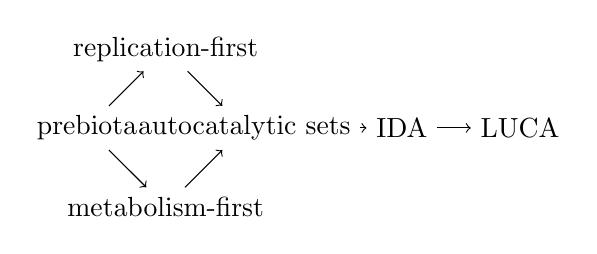
\begin{tikzpicture}
\node (prebiota) at (0,0) {prebiota};
\node (metabolism-first) at (1,-1) {metabolism-first} edge [<-] (prebiota);
\node (replication-first) at (1,1) {replication-first} edge [<-] (prebiota);
\node (acs) at (2,0) {autocatalytic sets} edge [<-] (replication-first) edge [<-] (metabolism-first);
\node (ida) at (4,0) {IDA} edge [<-] (acs);
\node at (5.5,0) {LUCA} edge [<-] (ida);
\end{tikzpicture}

Two alternative models exist for the step from abiotic to \gls{ida}: genetic or replicators or RNA-first, and metabolism or protein-first. Both metabolism and replication were almost certainly required for \gls{ida} however. A self-sustaining autocatalytic network (in terms of a RAF set specifically a ``set of molecules and reactions which is collectively autocatalytic in the sense that all molecules help in producing each other (through mutual catalysis, and supported by a food set).'') generally considered essential \parencite{Pross2013}, but not sufficient \parencite{Hordijk2011}. Both competing models--replication first and metabolism first--build on that. Autocatalysis expressed by self-replication of oligomeric compounds in replication first; by cycles and network in metabolism first. In the broadest sense, life can be seen as an autocatalytic process where an entity catalyses the production of one or more descendant entities.
From another perspective, Metabolism-first privileges function, while replicator-first privileges descent.

The main issues with replicator-first model are the sizeable step required from abiotic compounds to template-based replication (although ribonucleotides conceivably could form in pre-life conditions see \parencite{Powner2009}). Templates encode information in biology, so require a encode/decode mechanism as well as an information code to represent the product. This is a step more complex than simpler duplication. By contrast, the main issue with metabolism-first model concerns the shift from composome inheritance to template-based, and the ability of composomes to fulfill heredity requirement for natural selection.

The origin of life can be seen as the transition from chemistry to biology, and is analogous to our goal of transitioning from simple uninteresting systems, to systems which evolve. However, the usefulness of the similarity is limited: the primary postulates of OOL are not our postulates. Some abiogenesis results fundamentally assume real-world chemistry and
conditions, a constraint that doesn't apply to Alife or artificial OEE, and so is more restrictive than required. Other abiogenesis work such as on properties of autocatalytic sets, or the suitability of the genetic and catalytic properties of RNA for Alife \parencite{Cheng2010}, is broader in applicability.
\end{mdframed}

\paragraph{Living organisms are supremely well suited to their environments, and can adapt to environmental changes}

Adaptation of organisms to their environments occurs in the main on two different time-scales.

Evolution by \gls{naturalselection} acts over a period of generations on populations of individual organisms. Changes are therefore relatively gradual, and many generations can pass before a change such as a beneficial mutation becomes ubiquitous in a population (\eg 300-500 generations for targeted modifications in lactose processing in \emph{E. coli} \parencite{Dekel:2005fk}. In contrast, gene regulatory effects act during the life cycle of a single individual, either during development to affect morphology, or during the adult lifespan in reaction to seasonal or other environmental cues. These regulation-driven changes are not in themselves heritable, but they can be assimilated back into the population by influencing the organisms fitness under natural selection (\eg,\parencite{Baldwin:1896ly,Dennett:2003ve,Paenke:2009xe,Paenke:2007ve}).

Similar effects can be seen by another adaptive mechanism that operates on individuals during their lifespan: learning, where behavioural adaptions can also lead to genetic change (\eg \parencite{Hinton:1987vy}.)

\paragraph{Natural selection, acting on populations, is the primary driver for long-term adaptation}

The year 2009 saw the celebration of the 150\textsuperscript{th} anniversary of the publication of \emph{On the Origin of Species}, the explanation of evolution by natural selection, with extensive coverage in scientific and popular media. The terms are therefore fairly well known to many people, but what exactly does \emph{natural selection} mean? To quote from \parencite{Futuyama:1979tg}, \gls{naturalselection} is the ``differential survival and reproduction of genotypes''.

Let's examine each of the components in this idea in turn:

Differential survival. Living organisms are constantly engaged in an intimate relationship with their environments. Indeed, according to the theory of \emph{autopoiesis} \parencite{Varela:1974qd}, organisms are defined by this engagement: to be alive means maintaining oneself against the surrounding environment. In general the more effectively the organism is able to do this, the more likely it is to survive. However, in practice survival for an individual may be affected by random events. Scholarship winning students can be killed by drunk drivers. Sardines in shoals flash and turn, yet sharks still manage to grab one or two from the shoal effectively at random. Averaged over a population however these chance events balance out; a succession of random trials leads to a skewed distribution of fitness away from the less able.

Reproduction. In this sense, reproduction simply means inheritance. Only those characteristics that can be passed on from one generation to the next are relevant. One implication of this is that the only traits of an organism that matter to natural selection are those that are apparent while the organism can reproduce. Altruism and kin-selection, where an individual acts to increase the fitness of a related individual, are interesting for the light they shed on this implication.

Genotypes. An organism's \gls{genotype} is the heritable information that defines an individual, of which the great majority is encoded in DNA (some \emph{epigenetic} information is inherited through DNA-methylation, maternal protein concentrations and other mechanisms. However, generally DNA remains the primary source.)

How then does natural selection unfold in practice? Although an organism is defined by its genotype, its survival is based not on the raw genotype, but on the expression of the genotype--called the \gls{phenotype}--that participates in the interaction with the environment. There is not necessarily a direct one-to-one mapping between genotype and phenotype; for example, environmental triggers
during development can switch the phenotype in different directions (a phenomenon called \gls{polyphenism}.)

This indirect mapping enables a number of important mechanisms significant to the operation of natural selection: first, changes in the genotype (caused by mutations for example) may build up independent of phenotype changes--the idea of \emph{neutral mutations} \parencite{Ohta:1996vn,Ohta:2002ys,Ohta:1973kx}. Examples from studies of RNA secondary structures (the physical folding of RNA molecules) show that many closely-related RNA sequences can produce the same RNA folding \parencite{Fontana:1993zn}. Adjacent changes often have little effect on structure.

Second, by extension, \parencite{Gavrilets:1997qt} and \parencite{Gravner:2007yd} have shown that in cases involving many gene loci under well-defined conditions there is a path between viable phenotypes that requires only neutral mutations.

Third, behaviours such as learning, rather than purely genetic mechanisms, can influence the form of this \gls{gpmap} in combination with natural selection, as illustrated by the Baldwin effect \parencite{Baldwin:1896ly} and other examples of genetic assimilation \cite{Hinton:1987vy,Siegal:2002qn,Waddington:1942jb}.

Finally, a \gls{grn} provides another mechanism to modify the \gls{gpmap} and hence to guide natural selection.

\paragraph{Novelties often arise from new regulatory connections rather than changes to genes}

The phenotype in living organisms is many orders of magnitude more complex than the genotype, and the methods used during development to build this complexity are many and various.

Cells call upon a complex of regulatory processes to regulate the expression of genes, and hence to control development and morphology (as well as to implement the cell's basic machinery.) The majority of these processes (at current understanding) use proteins to affect the initiation of transcription (the production of RNA from a segment of DNA, the first stage of gene expression); most commonly the presence of a specific protein promotes or inhibits the transcription of a related gene, and without transcription the gene is silenced.

One step further along the protein production chain, editing and splicing of the RNA products of transcription in eukaryotes prior to translation (the production of a protein from mRNA) is also under regulatory control. Many alternative proteins from one transcript can be produced, triggered by environmental or other influencing factors; each alternative protein will have a different effect on cell function. As a result, in biological organisms, the phenotype is not uniquely determined by the genotype, and a genotype contains the potential for multiple different phenotypes under the influence of the environment (a phenomenon known as plasticity).

Patterns of gene expression can also have an effect outside the originating cell, a phenomenon crucial for development. Signalling proteins produced by a cell act as regulators on the machinery of surrounding cells, and epigenetic mechanisms allow signal effects to be long-lived so that a pattern of expressions may be inherited by daughter cells without the continued presence of the original signals. These mechanisms determine the fate of new cells during development: a cell originating in an area bathed in a particular combination of signalling molecules will develop in a specific manner (such as into a skin cell); another cell in another area will receive different signals, and therefore develop in a different way.

The development of an organism from a zygote is thus controlled by a pattern of gene expression under the combined influence of a regulatory mechanism and the environment.

As the regulatory mechanism is constructed from proteins and RNAs encoded in the genotype, and as the genotype is generally under the influence of natural selection, evolution also acts upon gene regulation, and hence upon development. The study of the evolution of the developmental mechanism itself is known as Evolutionary Development, or, more colloquially, EvoDevo.

\parencite{Prudhomme:2007ax} believe that evolutionary novelties more commonly arise from changes or additions of regulatory \emph{connections} than from the development of \emph{new} genes or regulatory elements; that is, from changes to the network topology rather than from additions to the network elements. The underlying implication is that novelties are therefore new compositions of
pre-existing elements, rather than being constructed `\emph{de novo}', and that production of novelties may be relatively rapid. Connection changes may happen quickly; by comparison, new genes may take many generations.

\begin{flushright}
	\emph{According to the strictly structural concept, the genotype is considered as a mosaic of independent molecular blue-prints for the building of individual cellular constituents. In the execution of these plans, however, co-ordination is evidently of absolute survival value. The discovery of regulator and operator genes, and of repressive regulation of the activity of structural genes, reveals that the genotype contains not only a series of blue-prints, but a co-ordinated program of protein synthesis and the means of controlling its execution.}
	\par\cite[p354]{Jacob:1961ys}
\end{flushright}

A network formed by the regulatory interactions between genes and the transcriptional products of those genes (\glspl{tf}) is known as a Gene Regulatory Network, or \gls{grn}.

\paragraph{Modularity is an emergent property of GRNs}
Even a superficial look at a set of randomly sampled insects reveals a striking level of similarity between supposedly distantly related species. Mouthparts, segmented bodies, wings and halteres springing from body segments, antennae on head segments; common patterns abound. The explanation lies in the action of a group of homeotic (or body-patterning) genes, which act in concert to impose a structure on the developing body plan. These regulatory genes, amongst the first patterning genes to be identified and characterised, in fact appear in very similar forms across all animals and hence appear to share a common evolutionary origin, and to be highly conserved \parencite{Shubin:2009vw}. 

As an example of their action, the gene \emph{Ubx}, or \emph{Ultrabithorax}, is involved in development of the \gls{metathorax}, one of the body segments, in \glspl{arthropod} \parencite[pg. 696-697]{Watson:2008fm}. Changes in \emph{Ubx} expression in combination with expression of a second homeotic gene, \emph{Scr}, are responsible for some of the differences in body plan between two arthropod groups--brachiopods, and isopods. In brachiopods, the expression of \emph{Ubx} suppresses \emph{Scr} in the leading thorax segment leading to development there of swimming legs. In isopods however, \emph{Ubx} expression has been lost in that segment, and instead a feeding appendage develops \parencite{Watson:2008fm}.

The morphological patterns that result from changes in expression of the \emph{hox} homeotic genes are textbook examples of modularity caused by regulatory networks. These networks in general appear to take a characteristic form, sometimes called a `medusa' network \parencite{Kauffman:2004zi,Aldana:2007da} where a regulatory head controls the expression of many functional genes. For example, in \gls{drosophila}, the medusa has a head of around 80 genes \parencite{Aldana:2007da}. \Textcite{Davidson:2006wi}, using the well-characterised sea urchin genotype, identifies GRN `kernels' of interconnected and hence very robust regulatory genes that control essential functions such as heart development and the endoderm specification in sea urchins. 

\subsection{Evolutionary principles from Biology}

``We take it as given that biology instantiates ENS'', but that doesn't mean that the algorithm of biology is in fact \gls{ens} \parencite{Watson2012}. Adaptation in biology appears to precede Natural Selection, so adaptation is possible without \gls{ens} \cite{Watson2010}. \cite{Saunders1994}, discussing Lovelock's DaisyWorld model, explains how regulation can emerge in DaisyWorld without selection--the planet's temperature is adjusted to meet the conditions for maximum growth of the daisies without the daisies adapting to the planet. In fact, \cite{Saunders1994}, referencing Mayr, comments that Darwin could not prove that \gls{ens} was the only mechanism for adaptation in biology, just the most likely one. Subsequently, the developing understanding of the biology in areas such as \gls{hgt} and neutral theory \cite{Kimura:1968uq} has enhanced the purely Darwinian view of \gls{ens} in natural populations into what is now generally referred to as the modern evolutionary synthesis.

Although the advantages of a distinction between genotype and phenotype are discussed by many, including \parencite[section 7.2.3]{Taylor1999} and indirectly \cite{VonNeumann1966}, there is no inherent dependency on this in \gls{ens}. Early evolution may have involved holistic or composomal evolution before the advent of digital evolution with a separate genome.

\quote{Evolution is a process that results in heritable changes in a population spread over many generations.}{
	``Sandwalk: strolling with a skeptical biochemist'',
	\url{http://sandwalk.blogspot.co.nz/2012/10/what-is-evolution.html}}

\quote{
	Biological evolution consists of change in the hereditary characteristics of groups of organisms over the course of generations. Groups of organisms, termed populations and species, are formed by the division of ancestral populations or species, and the descendant groups then change independently. Hence, from a long-term perspective, evolution is the descent, with modification, of different lineages from common ancestors.}{``Evolution, Science, and Society: Evolutionary Biology and the National Research Agenda'', Working Draft, 28 September 1998, \url{http://www.zoology.ubc.ca/~otto/evolution/Evolwhite.pdf}}


\subsubsection{Evolution by Natural Selection (ENS))}\label{ens-evolution-by-natural-selection}

\cite{Godfrey-Smith2007} examined a number of summaries of \gls{ens} in the literature. The purposes of the summaries varied, but have interest for us ``as attempts to capture some core principles of evolutionary theory in a highly concise way.''. Incidentally, as an illustration of the difficulty of definitions, although the usual aim is to ``give conditions that are sufficient ceteris paribus for a certain kind of change occurring.'', \cite{Godfrey-Smith2007} notes that the scope of most summaries is somewhat ambiguous. They can be read as either being discriminatory--``this process is ENS''-- or providing conditions that will result in \gls{ens} when it is assumed that the meaning of \gls{ens} is clear. In other words, these are alternative \emph{constitutive} or \emph{causal} readings; in the example of \cite{Godfrey-Smith2007}, ``becoming pregnant\ldots{}{[}versus{]} being pregnant'':

\begin{compactenum}
\item ``Owing to this struggle for life, any variation, however slight and from whatever cause proceeding, if it be in any degree profitable to an individual of any species, in its infinitely complex relations to other organic beings and to external nature, will tend to the preservation of that individual, and will generally be inherited by its offspring. The offspring, also, will thus have a better chance of surviving, for, of the many individuals of any species which are periodically born, but a small number can survive. I have called this principle, by which each slight variation, if useful, is preserved, by the term of Natural Selection, in order to mark its relation to man's power of selection.'' \cite{Darwin1859}

\item ``if there is a population of entities with multiplication, variation and heredity, and if some of the variations alter the probability of multiplying, then the population will evolve. Further, it will evolve so that the entities come to have adaptations....'' (Maynard-Smith, in \cite{Griesemer2001})

\item ``1. Different individuals in a population have different morphologies, physiologies, and behaviors (phenotypic variation). 2. Different phenotypes have different rates of survival and reproduction in different environments (differential fitness). 3. There is a correlation between parents and offspring in the contribution of each to future generations (fitness is heritable).'' \cite{Lewontin:1970mc}

\item ``...evolution will occur whenever and wherever three conditions are met: replication, variation (mutation), and differential fitness (competition)'' \parencite[quoting Daniel Dennett]{Ofria2004}

\end{compactenum}

From the study of the summaries, \cite{Godfrey-Smith2007} concludes that the core requirement for \gls{ens} is some ``combination of variation, heredity, and fitness differences'', although he identified a number of differences between the summaries. For example, the most commonly cited summary is \cite{Lewontin:1970mc}, but unusually that formulation states that ``fitness is heritable'' whereas typically phenotypic heredity (as appears in Lewontin's later 1980 summary) is stated as sufficient for a trait to evolve. 

These differences are also discussed in \parencite{Griesemer2001}, in particular with reference to the variations between Darwin's concept of inheritance in \cite{Darwin1859} which includes both heritability (a capacity) and inheritance (a process carrying the capacity); Lewontin, which stresses the heritability while assuming inheritance, and Maynard Smith's multiplication which is actually about inheritance; his heredity is both. \parencite{Griesemer2001}

Quite apart from these differences in interpretation, the major theoretical difficulty in a literal application of \gls{ens} to artificial systems is captured succinctly by \parencite{Griesemer2005}: ``Darwin's theory of evolution by natural selection is restricted in scope. One sense in which it is restricted is that it refers to organisms.'' Organisms are not defined, but the context and scope is clearly biological.

Pigliucci2008--``Is evolvability evolvable?''

\subsubsection{Compositional evolution}

In life, have \gls{hgt} \eg \parencite{Ochman2000}; \parencite{Watson2002} discusses compositional evolution and building blocks; \parencite{Pross2011} introduces Dynamic Kinetic Stability as a general principle underlying evolution, and proposes it as the driver for the origin of life.

\parencite{Arthur2009} investigates the evolution of technology, where evolution is used in the sense of \quote{all objects of some class are related by ties of common descent from the collection of earlier objects.}{\parencite{Arthur2009}} In general though, Arthur's compositional evolution does not attempt to understand life, but instead as a guide to achieving similar property in another domain, or in understanding similar processes in another domain \parencite{Arthur2009}.

Evolution in technology occurs by using earlier technologies as building blocks in the composition of new technologies, and these new technologies then become building blocks for use in later technologies, and so on. Arthur calls this ``combinatorial evolution.'' But what is the starting point? How is this regression grounded? Arthur proposes that the capture and harnessing of natural phenomena starts each lin\eg and provides new raw components for inclusion in later technologies.

Evolution is related to innovation: in fact, Arthur claims that by understanding the mechanism by which technologies evolve we will understand how innovations arise. In other words, innovations arise as the result of an evolutionary process, rather than de novo from the brain of a designer. Darwinian evolution, or natural selection, is not appropriate for technology. Arthur quotes from Samuel Butler's essay ``Darwin Among the Machines'' : ``{[}t{]}here is nothing which our infatuated race would desire more than to see a fertile union between two steam engines\ldots{}'' to illustrate the impossibility of slavish adoption of biological models.

The first obstacle to a more general scope is the existence of innovations such as the jet engine, laser, railroad locomotive, or QuickSort computer algorithm (to name Arthur's examples.) Innovations seem to appear without obvious parentage; they do not appear to be the result of gradual changes or adaptations to earlier technologies. Arthur's answer is to look inside the innovation and to recognise that each is made up of recognisable components or modules; the key lies in the nature of heredity in technology. Technologies are formed by combining modules of earlier technologies. These groupings start as loose assemblages to meet some new function, but over time become fixed into a standard unit (for example, the change in DNA amplification mechanisms from assemblages of laboratory equipment to standard off-the-shelf products.)

\parencite{Bourrat2015} comments that distributive evolution (where only the distribution of elements changes, as result of selection or drift) cannot result in novelties. Arthur's response is that novelty comes from incorporating new phenomena from the source, the natural world.

\subsection{Evolutionary Algorithms}

The field of \glspl{ea} originated in the exploration of abstract biological evolution, but rapidly diverged into problem-solving and optimization \cite{De-Jong:1993gy,DeJong2006}. The fundamental differences between the biological original and the modern canonical \gls{ea} include:

\begin{compactitem}
\item \Glspl{ea} search through a fixed space, and hence cannot surprise by 'kind', only by 'degree' (\eg \parencite{Nellis2014})
\item The evolutionary process in an \gls{ea} is not itself subject to evolution; it is designed, and a large body of literature exists to guide the implementor in the choice of algorithms to employ.
\item Fitness in an \gls{ea} is measured by an explicit \emph{objective function} whereas in biology fitness \emph{emerges dynamically} through continuous interaction with the environment. ``The difference is that we require a system with the potential for a large degree of intrinsic adaptation for open-ended evolution, rather than a system where the selection of individuals is determined by an externally-defined fitness function'' \parencite{Taylor2001}
\item \Glspl{ea} conduct a series of discrete trials of fitness, rather than a continuous evaluation.
\item Individuals in a \gls{ea} do not interact other than indirectly through a pre-designed selection mechanism.
\item \Glspl{ea} are not dynamical systems unlike the biological origina. Dynamics required for novelty-generation \parencite{Nellis2012}
\item Natural organisms must replicate themselves to pass on genetic information--``final arbiter of fitness'', and interaction with other organisms and with environment \parencite{Ofria2004}
\end{compactitem}

The first two of these differences are significant; \glspl{ea} are not capable of open-ended, or evolutionary, evolution. However, recent research in biology continues to be applied to improve the performance of \glspl{ea} in their core function of optimization:
\begin{compactitem}
	\item Redundancy and degeneracy--\eg \parencite{Whitacre:2010qy}
	\item Novelty--\eg novelty search \parencite{Lehman:2008cr}
	\item EvoEvo, or the evolution of evolution--\eg the remainder of this work.
\end{compactitem}

For example, a summary of some relevant work in the application of \glspl{grn} to \glspl{ea} to improve the robustness and modularity of solutions can be found in \ref{applications-of-grn-in-eas}.

A form of re-unification between biological evolution and artificial evolution has been attempted in works such as \parencite{Paixao2015}, based on \quote{models in theoretical population genetics and in the theory of evolutionary computation}{\parencite{Paixao2015}}. For example: \quote{Some EDAs can be regarded abstractions of evolutionary processes: instead of generating new solutions through variation and then selecting from these, EDAs use a more direct approach to refine the underlying probability distribution. The perspective of updating a probability distribution is similar to the Wright--Fisher model.}{\parencite{Paixao2015}}

\section{Guide to this work}

\section{Previous publications}\label{previous-publications}

A version of Reactant and Product Strategies \cref{reactant-and-product-strategies} was published as \cite{Young2015},
and material from \cref{model-validation} in \cite{Young2013}.

ToyWorld is available under an GNU GPL v2 open source licence from GitHub \cite{toyworld}.

\section{Contributions}\label{contributions}

\begin{compactenum}
\item Open-sourced Artificial Chemistry model
\item Progress towards useful heredity in an artificial system
\item Progress towards OEE in artificial system--evolution compatible with OEE without necessarily showing OEE (which is hard to measure and prove)
\item Demonstration of formation of ACS in an artificial chemistry (previous work with ODEs e.g. \parencite{Hurndall2014} not re-usable in that form)
\end{compactenum}

\chapter{Previous work}\label{previous-work}

\epigraph{%
	It may appear that the properties one would have to assign to a population of self-reproducing elements in order to obtain Darwinian evolution are of a spectacular simplicity. The elements would only have to: (1) Be self-reproducing and (2) Undergo hereditary changes (mutations) in order to permit evolution by a process based on the survival of the fittest.}%
{\textit{\\Nils Barricelli}\\\textsc{Cited in \cite{Taylor2001}}}

Emergent systems easy to code but produce surprising results. Cannot predict results from rules (or in fact easily predict rules from desired results. One-way function, akin to encryption) \parencite{Nellis2014}

Much of this work falls under the banner of \gls{alife}, both weak and strong as distinguished by \cite{Langton1989}: ``study the phenomena of life, not by simulating life as it is (weak AL) but by instantiating life as it could be (strong AL)''

First, a distinction: open-ended evolution refers to a goal or result, while evolution-of-evolution, or EvoEvo, describes a process or mechanism. The first is constitutive, the second causal. In artificial systems, the most influention formulation of the problem overall remains that of \cite{Bedau:2000mi}:

\quote{A key challenge is whether digital systems based on symbolic logic harbor the same potential for evolutionary innovation as physical systems. A preliminary challenge is to unlock the full potential of evolution in digital media. Many believe that digital life today falls far short in this regard, and this issue is starting to be approached quantitatively.}{\cite{Bedau:2000mi}}

Previous work falls into five specific areas:
\begin{compactenum}
\item Constitutive definitions of open-ended evolution--part of the problem definition, and hence in the Introduction, \ref{}
\item Causes of open-ended evolution
\item Theoretical basis for copy mechanism--extracted into the Previous Work section of \ref{} as it is a major contribution.
\item Systems that implement the specific elements we support
\item Systems that are capable of these elements, but are missing one (the copy mechanism)
\end{compactenum}

\section{Replicators and inheritance}

We're interested in heredity and inheritance, which in biology is tied to the concept of a replicator. Dawkins first to define replicators--includes genes, memes. Many other definitions and formulations followed as various properties or features examined in subsequent works. Relatively recently, \cite{Zachar2010} saw a need to rexamine the definition primarily to resolve issues of discrimination between entities which are clearly replicators or not replicators, and those which are borderline, and between biological replicators and non-biological or cultural ones. In summary,

``Replicator: any autocatalytic entity for which there is a selection process defined. Selection is a process, acting on a particular population of entities in a particular environment, which sorts entities according to their phenotypes.'' \parencite[p.21]{Zachar2010} (terminology slightly different in Bourrat2015--persistors, replicators, reproducers...)

''A regenerating/recreating entity can produce at least
one entity equivalent to it. It is possible that the original
entity immediately decomposes (that is, cannot be the
subject of further turns of the cycle), causing sequential
replacement, although this is the most simple of regenerating
entities. If it can effectively increase the number
of entities equivalent to itself, then it is autocatalytic
and is a \emph{replicator}. The simplest of replicators is the
\emph{exact replicator}, which is \emph{non-informational}, and any
change made to it causes a change in the phenotype. If
a variation can arise in the structure in such a way that
it does not change equivalence of the entity, then it is a
\emph{variable} replicator, with more than one stable state. If
such changes can be passed on to the offspring then the
replicator is \emph{informational}. If the non-heritable part is
constructed by a developmental process, then the replicator
is a \emph{reproducer}.'' \parencite[p.21]{Zachar2010}

Autocatalysis by definition is replication--the autocatalytic reaction $x+A->2A$ replicates the molecule $A$ \cite{Lifson1997}--applied at first to molecules. Only variation through mutations (unless alternative reaction products/networks, but even then restricted to a small set of alternatives by catalytic structure. Stoichiometrics not so significant in ACS/linear growth overwhelmed by exponential dynamics of catalysis.)

Heredity by \cite{MaynardSmith1999} is modular or holistic--if module changed only that module changes in descendants, holistic change part changes whole. Believe it true that unlimited heredity => modular. \cite{Szathmary1999} calls these digital and holistic, and adds phenotypic replicators whereby ‘phenotype or function of one object is translated to the other, without any modular copying effect” (how does this differ from holistic?)

\cite{Hogeweg1997} describes attractor-based heredity (inheritance of state) and storage-based. 

\cite{Vasas2012a} ACS cores are attractor based, DNA/RNA storage based. HGT/LGT--compositional inheritance.
Difficulties with Compositional inheritance in something like GARD where just a correlation between parent and child--response to selection not seen \parencite{Vasas2015}--end up with just one large component (so no selection), no replication as contents not inherited equally, so properties might be quite different from parent. Information fidelity varies widely. Mutations in cycles \parencite{Vasas2012a} generally not heritable as mutant copies generally not functional in autocatalysis. So problem with mutations as source of variation. Alternative to mutations is avalanches--form new cycles from side-products.
But can see heredity in autocatalytic cores (one or more linked autocatalytic loops) as a form of genotype--any molecule in core will produce remaining species in core and periphery \parencite{Vasas2012a}. Core forms an attractor; one core=one attractor, and no evolution possible as no selection. Multiple cores (from inhibition \cite{Vasas2012a})=multiple attractors, but need attractors to be stable for stable selection. Cores are equivalent to one-bit of heritable information, so hard to see as unrestricted heredity as limits to numbers of cores…
\cite{Watson2015} summarizes two forms of inheritance for groups, being either ``migrant pools'', where members disperse horizontally to form new pools, or group fissioning, where the dispersion is vertical. Fissioning, in the view of \cite{Watson2015}, provides for group inheritance whereas migrant pools do not.

Modular/template heredity has advantages of: mutations hereditary; problems of correct copying \parencite{Eigen1977}

Selection implies limits on fidelity--at least one perfect copy on average at each replication required \parencite{Eigen1977}

\section{Systematic Map}

Purpose: to identify gaps in current research. Summary of research area required to ensure 1) outline where proposed work fits into existing body of knowledge 2) do not repeat previous work 3) identify future research directions

Research Method: the method is a Systematic Map. Evidence-based. Derived from Evidence-based medicine (see \cite{Cochrane:2011qy, CRD:2008fj}). Primary motivation is to remove unintended bias in reviews; also can quantify consistency or variation in subject \parencite{Kitchenham:2007nx}.
Major differences with standard expert-review is in pre-definition of research protocol, search strategy, exclusion and inclusion criteria, quality criteria. All documented so can be repeated, or at least, given the difficulty of repeating a digital library search, at least evaluated by other researchers and practitioners.
\subsection{Need for a review}

Two previous reviews are known of the general topic: \cite{Duthen2010} and \cite{Stanley:2003fh}.

\Textcite{Duthen2010} is a survey of artificial creatures, examining on the mechanisms used rather than the problems or goals addressed. Research is grouped by environmental simulators, means to assemble creatures from pieces (phylogeny) and 
ways to generate creatures from a seed (ontogeny).

\Textcite{Stanley:2003fh} opens with a mini-review of Artificial Embryology.
Discounted the value of the traditional distinction between grammatical and chemical encodings, and went on to propose a five-part taxonomy
instead--cell fate, targeting, heterochrony, canalization and complexification--based on biological research. Quite
biological in basis, and some aspects of the taxonomy seem prescriptive (\eg cell fate).

Otherwise, no specific reviews of Developmental Encodings known (search 20 June 2012 of Web of Science with search string
(TI=("Morphogenesis" OR "Embryogeny" OR "Artificial Embryogeny" OR "Developmental" OR "Generative Representation" OR
"Evolutionary Development")) AND Document Types=(Review)--3,713 results found, but neither of the two in Computer
Science are relevant. Note that this search doesn't retrieve either known review: \cite{Stanley:2003fh} is labelled on WoS as an
"article" rather than as a review, and \cite{Duthen2010} references ``Artificial Creatures''. Removing the "review" condition returns 76,708 results.

\subsection{Method}

\subsubsection{Research questions}
Our objective is to confirm the range of previous work by supplementing the identified papers by a systematic selection.

\begin{enumerate}[label=RQ\arabic*:]
	\item What previous work in Artificial Life specifically discusses inheritance or heredity in artificial chemistries?
\end{enumerate}

\subsubsection{Systematic Reviews and Maps}

Maps are exploratory (``what is known about X?'') while Reviews address specific research questions (``Is procedure X more effective than procedure Y for outcome O in context C?'')
For Maps, ``The main goal of a systematic mapping studies is to provide an overview of a research area, and identify the quantity and type of research and results available within it. Often one wants to map the frequencies of publication over time to see trends. A secondary goal can be to identify the forums in which research in the area has been published.'' \parencite{Petersen:2008fk}
For Systematic Reviews, \cite{Kitchenham:2007nx} recommends research questions address five criteria: population (those affected), intervention (method or technology under investigation), comparison (control method or technology), outcomes (factors or elements of comparison), context (in which the comparison takes place)

Systematic Map \parencite{Petersen:2008fk}, rather than Systematic Literature Review \parencite{Kitchenham:2007nx}. According to Petersen's set of differences between Reviews and Maps, we less interested in the state of  evidence rather than classification; less emphasis on assessing the quality of the primary studies; a broader focus; stronger emphasis on breadth rather than depth of review.

Systematic Maps also provide categorisation of a research area, but this is not the main goal of the process. Instead a Map uses the generated classification as a framework for further analysis, summarising contributions by category. However the processes are similar in that one process for categorisation in Maps \parencite{Petersen:2008fk} extracts keywords from the paper abstracts and iteratively groups and refines these into the final categories.

Note that both Reviews and Maps usually rely exclusively on Primary sources (originals) rather than Secondary (interpretation, or after-the-fact), or Tertiary (distillation or collections of Primary and Secondary sources)

\subsubsection{Research team and decision procedure}
RQ1: what previous work exists for inheritance or heredity in artificial chemistries?
RQ2: who are the main researchers, and what research communities exist?

One reviewer only (PhD thesis limitation). 

Quality checks by 1) confirm that search identifies previously known papers 2) check-recheck at different dates or blind sample rechecked and kappa statistic calculated 3) confirm decisions with supervisor 4) send form to paper author for notice if incorrect?

\subsubsection{Inclusion and exclusion criteria}
Inclusions: Primary research

Exclusions: Reference works,biological modelling,  education, introductions, summaries of research, case studies, application of research, Keynote abstracts, programming paradigms, computer art, biology, software engineering, genetic programming and algorithms

\subsubsection{Stage 1--Source selection}

\begin{table}
	\footnotesize
	\begin{center}
		\begin{tabular}{@{}p{5cm}p{8cm}@{}}
			\toprule
			Data source & Rationale for inclusion\\
			\midrule
			IEEE Xplore & Major computer science database and proceedings for \textit{IEEE Congress on Evolutionary Computing}\\
			ACM Digital Library & Major computer science database and proceedings for \textit{GECCO}\\
			Springer & Proceedings of \textit{ECAL}, \textit{CompLife} and \textit{Parallel Problem Solving from Nature conferences}\\
			Web of Science & Broad coverage, multiple fields\\
			Previous primary studies & Quality and consistency check\\
			References and citations from previous primary studies & Likely to be relevant \\
			\bottomrule
		\end{tabular}
	\end{center}
	\caption{Data sources}
\end{table}

No journals were directly included as \textit{Artificial Life} and \textit{Adaptive Behavior}, the two principal journals in the Artificial Life field \cite{Aicardi2010}, are indexed by \textit{Web of Science}. No general internet search was performed. 

\subsubsection{Stage 2--Keywords}

"artificial chemistry" AND (inheritance OR replicator OR template OR holistic OR reproduction OR reproduce OR heredity OR composome)

\subsubsection{Stage 3--Automated Search}

Publication bias--tendency of published papers to support hypothesis, reject null hypothesis. Papers which do not less likely to be published. Address by 1) awareness 2) grey literature search 3) funnel plot of variance against effect--expect higher variance for small samples

\begin{table*}
	\footnotesize
	\begin{center}
		\begin{tabular}{@{}p{2cm}p{2cm}p{9cm}@{}}
			\toprule
			Datasource & Query & Results\\
			\midrule
			ACM Guide to Computing Literature & (+"artificial chemistry" inheritance replicator template holistic reproduction reproduce heredity composome)&73 records\\
			\midrule
			IEEE & "Abstract":“artificial chemistry” AND (“inheritance” OR “replicator” OR “template” OR “holistic” OR “reproduction” OR “reproduce” OR “heredity” OR “composome”)&6 records  \\
			\midrule
			Web of Science & (TS=("artificial chemistry" AND (inheritance OR replicator OR template OR holistic OR reproduction OR reproduce OR heredity OR composome))) AND LANGUAGE: (English)&26 records\\
			\midrule
			SpringerLink (via JabRef) &"artificial chemistry" AND (inheritance OR replicator OR template OR holistic OR reproduction OR reproduce OR heredity OR composome) & 129 records\\ 
			\bottomrule
		\end{tabular}
	\end{center}
	\caption{Query parameters for search 3a. Searches were not restricted to any year range.}
\end{table*}

SpringerLink search syntax difficult to structure exact same query; acceptable, but returns many false positives.
\subsubsection{Stage 4--Screening on title}

Combine all entries, and remove duplicates. 81 entries remaining.

Quality check--did we rediscover the papers we'd found earlier by expert search? And if not, why not?
\begin{table*}
	\footnotesize
	\begin{center}
		\begin{tabular}{@{}p{2cm}p{9cm}@{}}
			\toprule	
			Literature & Result \\
			\midrule		
			Avida \cite{Ofria2004}&No.\\
			Tierra \cite{Ray1991} &No.\\
			\cite{Nellis2012}\cite{Nellis2014} & No--abstracts reference embodiment and novelty but not inheritance and heredity.\\
			StringMol \cite{Hickinbotham2012}   & No, but similar found.\\
			\cite{Fontana1992}	& No--abstract doesn't reference inheritance or heredity, but focusses on function composition and patterns.\\
			\cite{Dittrich1998}	& No, but similar found.	\\
			\cite{Nowostawski2005} & No.\\
			\cite{Fenizio2000}\cite{Fenizio2001} & Yes.	\\		
			NAC \cite{Suzuki2006}    & No, but similar found.\\
			\cite{Gardiner2007}  & Yes.\\
			\bottomrule
		\end{tabular}
	\end{center}
	\caption{Rediscovery of existing key papers.}
\end{table*}

\subsubsection{Stage 5--Screening on abstract}
Difficult to be error-free; preference is therefore not to exclude based solely on abstract, although this does increase the workload.
Based on this, justified all exclusions and inclusions that were borderline. Clear inclusions and exclusions were not justified.

58 records after abstract screening.

Issues:
\begin{itemize}
	\item Ambiguous terminology--many fields have common terms \eg map, evolve, generative
	\item Insufficient detail in abstract
	\item Downloading abstracts at time of initial title search so don't have to re-search after initial selection
	\item Depth or degree--difficulty in determining the degree of focus on generative ideas from the abstract. If a paper mentions generative ideas amongst other exclusion considerations, is the paper included or excluded?
	\item Database specifics--inability of SpringerLink to correctly apply date limits in searches; difficulty in SpringerLink and ACM to batch-download citations--one at a time leads to fatigue and error. ACM bibtex export does not export abstract--must cut and paste. 
\end{itemize}

\subsubsection{Stage 6--Removal of duplicates}

Removal of exact duplicates--same publication source, title, authors. Performed as part of Stage 4 using JabRef's duplicate feature to identify potential duplicates. Unfortunately the algorithm appears to be case-sensitive, and so didn't detect some potential duplicates that were then identified in a follow-up by inspection.
Removal of likely duplicates--difficult however to judge conclusively from abstracts alone if two papers do describe the same research. However, this case didn't occur in our dataset.

\subsection{Results}


\subsection{Synthesis, analysis and discussion}

Sensitivity analysis--remove poor quality or subjective papers or particular type of paper and compare results.

\subsection{Limitations}
Subjective assessment of papers from title and abstract--may miss some relevant studies based solely on quality of abstract.

\todo{name for evolutionary replicators--Zachar?}

\begin{sidewaystable}
	\begin{center}
		\scriptsize
		\caption{Previous work}
		\label{tb:previous-work}
		\begin{tabular}{@{}llll@{}}
			\hline\noalign{\smallskip}
			\Gls{achem}                                                     & Type 	& Notes\\ 
			\\ \noalign{\smallskip}
			\hline
			\noalign{\smallskip}
			
			Avida \cite{Ofria2004}                                  		&Assembler Automata&	& Embedded copy algorithm\\
			Tierra \cite{Ray1991}                                  			&Assembler Automata&	& Embedded copy algorithm\\
			\cite{Nellis2012}\cite{Nellis2014}								&Boolean Networks and Graphs&&\\
			StringMol \cite{Hickinbotham2012}                             	&Rewriting or String-based&&\\
			\cite{Fontana1992}												&Rewriting or String-based&&2-parent function\\
			\cite{Dittrich1998}												&Rewriting or String-based&&2-parent function\\
\hline
			\cite{Nowostawski2005}											&&&\\		

			\cite{Fenizio2000}\cite{Fenizio2001}							&Rewriting or String-based&&\\			
			NAC \cite{Suzuki2006}                                         	&&&\\	
			\cite{Gardiner2007}                                             &&&\\
\hline			
			\cite{Kauffman1986}												&Compositional&&\\
			Turing															&Rewriting 	&&Yes\\
			Von Neumann														&&&\\
			Waddington														&Biology&&\\
			\hline
		\end{tabular}
	\end{center}
	\caption{Achems with evolutionary replicators.}
\end{sidewaystable}

\begin{sidewaystable}
	\begin{center}
		\scriptsize
		\caption{Previous work}
		\label{tb:previous-work}
		\begin{tabular}{@{}llll@{}}
			\hline\noalign{\smallskip}
			\Gls{achem}                                                     & Type 	& Notes\\ 
			\\ \noalign{\smallskip}
			\hline
			\noalign{\smallskip}			
			ZChem \cite{Tominaga2004}                                     	&&Not self-referential--recombination rules are defined separately from objects\\
			Substrate-Catalyst-Link (SCL) \cite{Varela:1974qd,Suzuki2008} 	&&Not self-referential--recombination rules are defined separately from objects\\
			GGL/ToyChem \cite{Benko2003,Benko2005}                        	&Atoms/Molecules&&None--at level of reactions\\			
			Squirm3 \cite{Hutton2002,Hutton2007,Lucht2012}                	&Atoms/Molecules&Replication by predefined reaction rules (not embedded)&\\
			RBN-World \cite{Faulconbridge2011}                            	&Boolean Networks and Graphs& None--at level of ACS\\
			\cite{Vasas2015, Vasas2012, Vasas2012a}							&Compositional&Non-template: Autocatalytic core-based inheritance\\
			\cite{Segre1998}												&Compositional&Non-template: Composomal\\
			\cite{Fernando:2008xy,Fernando:2007pf}                          &Compositional&Non-template: Lipid aggregates\\
			Lattice Artificial Chemistry \cite{Ono2000,Madina2003}        	&&&Non-template\\
			\hline
		\end{tabular}
	\end{center}
	\caption{Achems with non-evolutionary replicators.}
\end{sidewaystable}

\section{Copy-based approaches to the evolution-of-evolution in artificial systems}

Tierra \parencite{Ray1991}

Organisms had to allocate memory first before using. Initial selective pressure only from rate of replication. Sequential execution of organism code. \parencite{Ofria2004}

In Ray's words, ``...this approach involves engineering over the early history of life to design complex evolvable organisms, and then attempting to create conditions that will set off a spontaneous evolutionary process of increasing diversity and complexity of organisms''\parencite{Taylor2001}. The problem with `engineering over' is we don't understand the natural examples well enough to engineer them \parencite{Taylor2001}

Mutations are introduced during replication by randomly flipping bits during the copy operation (at a given rate of generally between 1 bit flip per 1,000 and 2,500 instructions copied). This rate is set by the experimenter, and is not evolvable. Mutations can also be introduced by the copy algorithm itself however; as it is an algorithm defined in the organism in standard Tierra instructions (and hence fulled embedded), mutations in the algorithm during a copy will be inherited by the child. The initial copy algorithm is part of the 80-instruction ancestral creature documented in \cite[app.C]{Ray1991}.

Emergence claimed in the three forms of \cite{Cariani1991}.

\todo{SugiuraSuzukiShioseEtAl2003}

Avida \parencite{Ofria2004}
``An approach to studying evolution...''

Avida summer of 1993--Tierra based with better metering and measuring, and parallel code execution.

Phenotypes--``The primary mode of environmental interaction is by inputting numbers from the environment, performing computations on those numbers, and outputting the results. The organisms receive a
benefit for performing specific computations associated with resources''

``In principle, the only assumption made about these self-replicating automata in the core Avida software is that their initial state can be described by a string of symbols (their genome) and that they autonomously produce offspring organisms. However, in practice our work has focused on automata with a simple von Neumann architecture that operate on an assembly-like language inspired by
the Tierra system.''
Instruction, read, write, and flow control heads for relative rather than absolute addressing--bit like a Turing tape machine. Many instructions grouped into instruction sets. Default set has 26 instructions, and by definition every program is valid.

New organisms are created asexually by the parent first allocating memory for a child. The parent's read-head is then placed at the beginning of its code, write-head placed at the start of the newly allocated memory and successive h-copy instructions copy the instruction from the read-head to the write-head and advance both. Either once all instructions have been copied (or perhaps before) h-divide splits the child from the parent (all instructions between read-head and write-head go to the child) and starts both executing in a clean state. Variation is introduced through mutations which can be introduced through either h-copy (the write-head writes a random instruction rather than the instruction at the read-head) or in h-divide (a single random instruction may be deleted or added from the child code). Both forms of mutation happen with a fixed probability set by the inventor: COPY\_MUT\_PROB, INS\_MUT\_PROB, and DEL\_MUT\_PROB for h-copy, and DIVIDE\_INS\_PROB, DIVIDE\_DEL\_PROB for h-divide. However, there is a second, evolvable source of mutations during replication--the replication process itself is embedded in the organism, as a set of instructions, and so changes to this algorithm during the copy will persist in the child. The self-replication algorithm is initially defined in the ancestral organism used to seed a run, and as documented in \cite[A1.3]{Ofria2004} consists of 15 instructions.

``The quest to halt adaptation is only one example of a special feature in Avida; many more have been explored, and are continuously being added to the source code. The most successful features are all fully described in the documentation that comes with the software.''

All very configurable, and complicated, but why? What rationale behind choices? More of a testbed for experiments, \eg `` in one experiment we wanted to study a population that could not adapt, but that would nevertheless accumulate deleterious or neutral mutations through drift''

\cite{Dittrich1998}:
A simulation approach towards ``dynamic phenomena, especially on the emergence of prebiotic evolution'', based on an artificial chemistry.

Introduction of \textless{}\emph{S},\emph{R},\emph{A}\textgreater{} classification scheme for artificial chemistry, elaborated in \parencite{Dittrich:2001zr}, where in this work \emph{S} are `` binary strings with a constant length of 32 bits'', \emph{R} are of the form $s1+s2 \rightarrow s3$, and \emph{A} ''simulates a well-stirred tank reactor with mass-action kinetics, which assures that the probability of a collision is proportional to the product of the concentration of the colliding objects'' (based on earlier work by Fontana and Kauffman.)

A=``1. Select two objects s1,s2 from the soup randomly, without removing them. 2. If there exists a reaction s1 + s2 to s3 and the filter condition f (s1,s2,s3) holds, replace a randomly selected object of the soup by s3.'', s1 and s2 are not consumed, rather they act as catalysts. Chosen as this shown capable of hypercyclic organisation

Asn automata reaction with a set of operations (six common logic operations, \eg OR, and nine computational instructions), represented as 4-bit sequences, to generate s3 from s1, s2. Automata is a deterministic FSA, running s1 on s2 to produce s3. As Dittrich observes ``The first noticeable property is that the structure of the product s3 is similar to its 'parents' s1; s2. This indicates that there is a correlation between s1, s2, and s3 that is a prerequisite for evolution.''

Passive self-replicators ($s1 + s2 \rightarrow s2$) are relatively common (approx. 30\% of randomly generated strings), while active self-replicators ($s1 + s2 \rightarrow s1$) are very rare (around 0.004\%).

StringMol \parencite{Hickinbotham2011}



GraphMol \parencite{Nellis2012} PhD thesis, and \parencite{Nellis2014} (summary of thesis)

``Our aim is to improve novelty-generation algorithms by making their biological models richer''

Computational novelty through embodiment. Comparing StringMol and GraphMol
Novelty-generation as goal/theme for meta-evolution. No measure for novelty--not even sure is possible. But informal definition that says more novelty as result of more embodiment (this seems circular?) p87 Embodiment as mechanism. 

Operates (like StringMol) at level of proteins/enzymes \eg replicases, DNA, genotypes, template copying.

Design is graph based. ``The world defined by GraphMol contains chemicals (represented as graphs) that bind to each other via multiple binding sites, and then run simple computer programs (encoded in the graphs) that modify the binding of these chemicals.''. Why? No explicit rationale presented. Presumably StringMol starting point meant programs, copying, then graphs? 

States that binding model needs to be rich--empirical evidence presented (StringMol) only
Runtimes in weeks to months.

Template copying refers to process of copying genotype from one generation to the next (imperfect digital copying as opposed to analog or compositional copying).

Mechanism of evolution must be itself evolvable; functions such as template copying must be embodied mechanisms in the world--so can be affected and evolved.
Individuals and environment interact to give new ways of producing new individuals.
Stringmol and Graphmol have embodied template copying, done in different ways. Different computational models result in different properties--``Stringmol exhibits macro-mutation and two chemical copying; GraphMol exhibits two types of quasispecies, cooperative and parasitic. These two systems use the same domain (emergent evolution) and metamodel (machines copying strings), but different computational models.''

General algorithm for template copying, used in both StringMol and GraphMol: \cite{Nellis2014}
i := start(string B)
while i not at-end(string B) do
string A(i) := char-copy(string B(i))
i := next(i)

Each of these four functions--start, at-end, char-copy, next--can either be ``crisp'' (i.e. perfect) or embodied (variable, the subject of evolution). Replicases are elements in the population that can copy themselves using this algorithm.

Copying is a phenomenon, expressed through mechanisms at different levels of the AChem. Explored through embodied copying mechanism built in GraphMol, with antecedent in StringMol \parencite{Hickinbotham2011}
StringMol includes an embodied start and at-end, crisp next, and stochastic char-copy. 

GraphMol has embodied start, at-end and next, with crisp char-copy. At-end uses Smith-Waterman matching algorithm, which opens ability for evolution to modify the function of at-end \parencite[p.143]{Nellis2012}. 

\subsubsection{EvoEvo Project}
The EvoEvo project (\url{http://evoevo.liris.cnrs.fr/about-evoevo-project/}), an Information and Communication Technologies initiative funded by the European Commission, begins at a higher level biological starting point (genotype-phenotype mappings). The project presupposes microbial evolution, ``at the level of genomes, biological networks and populations.'', with a focus on four specific properties of a genotype-phenotype mapping--Variability, Robustness, Evolvability, Open-endedness. Later work is planned to remove the biological specificity to provide a framework for applying EvoEvo to ICT problems. Along with development of a model founded on the ``genotype-to-phenotype mapping and the fitness landscape'', the project states that make use of \emph{Aevol} \parencite{Knibbe:2006vn,Knibbe:2007kx} to model developmental processes in microorganisms.

\emph{Aevol} describes the genotype-phenotype map of an artificial organism modelled closely on a prokaryotic cell. The genotype is therefore made up of a \emph{double-stranded circular} bit-string with genes marked by promotor sequences and terminated by sequences that can form a ``stem-loop'' structure (where bases are arranged in sequence along a protein such that the binding between complementary bases causes a characteristic loop to form in the protein.) Expression levels of a gene are based on the degree of similarity between the gene's promotor sequence and a predefined ``consensus'' sequence (as calculated by the Hamming distance), as is the case in real-world prokaryotes where the basal transcription level depends on the quality of the promotor \parencite{Sanchez-Dehesa:2008uq}. Translation in \emph{aevol} takes place between marked regions of the gene, and proceeds three-bit codon by codon, with each codon translated according to an artificial genetic code into an amino-acid equivalent in a protein.

The \emph{aevol} model contains several innovations:

\begin{compactitem}
	\item \emph{aevol} includes a proteome abstraction in the model in addition to the usual genotype and phenotype. Proteins in \emph{aevol} describe abstract ``processes'' instead of chemical interactions, where a process is described by a triangular probability distribution over $\mathbb{R}$ (in practice $[0,1]$ representing all processes) where triangles with positive height enhance the process and negative height processes act as inhibitors. The proteome then may be represented as either the superimposition of all protein distribution, or as the network of their ``functional interactions'' (the overlap between two protein distributions.) Note that the range of a process (protein) is equivalent to \gls{pleiotropy}; genes with a small range are functionally specialised. The phenotype of the organism is then the set of all positive processes (as calculated by Lukasiewicz fuzzy operators); that is, all activated but not inhibited processes.
	\item Mutations are not only the usual point-mutations (small deletions and insertions) but also \emph{genotype rearrangements}: deletions, translocations, inversions and duplications that act on a larger-scale.
	\item The environment for selection is also modelled by a similar distribution over $\mathbb{R}$. The closer the match between the organisms phenotype (as described above) and the environment distribution, the fitter the organism. This marks the full extent of environmental interactions in \emph{aevol} however. 
\end{compactitem}

To study the relationship between regulatory processes and adaptation to changing environments \parencite{Sanchez-Dehesa:2008uq}, two major changes have been made to \emph{aevol} to give \emph{RAevol} or Regulatory \emph{Aevol} \parencite{Beslon:2010zr,Sanchez-Dehesa:2008uq}. The first is the implementation of a fine-grained time model; proteins concentrations now vary dynamically (instead of remaining static as in \emph{aevol}), and the organism's proteome and phenome change over time to reflect these protein changes. The other is the addition of a regulatory model. The calculation of the basal expression level of a gene in \emph{RAevol} is the same as that in \emph{aevol}--a function of the Hamming distance between consensus sequence and gene promotor sequence. However, in \emph{RAevol} this level is modified by the action of regulation, either up-regulating or down-regulating the basal expression. The degree of regulation is determined by the concentration of proteins that may bind to two regulatory sites (an enhancer site and an operator site for inhibition) each 20-bits long. The ability of a protein to bind to the binding site is calculated from a predetermined ``affinity'' matrix that mediates between the DNA bit-string representation of the binding site, and the amino-acid representation of the protein. A simple process change in \emph{RAevol} enables interaction with the environment:  during simulation, a signalling protein of set sequence that has no metabolic function but can act as a \gls{tf} is sent to the organism when the target environment changes.

\section{Other potentially open-ended artificial chemistries}
Might be capable of EvoEvo, but either not demonstrated, or not a focus of the work. Meet the criteria other than demonstration of an evolvable copy mechanism.

\subsection{Assembler Automata}

Steen Rasmussen inspired by computer game core war--competing segments of simplified assembly code in core memory. With change to copy command to introduce mutations and hence evolutionary potential,
core world created: ``In the original core war game, the diversity of organisms could not increase, and hence no evolution was possible. Rasmussen then designed a system similar to core war in which the command that copied instructions was flawed and would sometimes write a random instruction instead on the one intended. This flawed copy command introduced mutations into the system, and thus the potential for evolution.'' \parencite{Ofria2004} 
But system ``collapsed into a non-living state'' {[}non-living?{]} One possible reason--copying over existing organisms \parencite{Ofria2004}

Tierra followed in the next year (relationship not stated) \parencite{Ofria2004}


\parencite{Taylor2001}:
Derived from Thesis (Taylor:1999sc): creation of \gls{alife}, Extension of Tierra \cite{Ray1991} by cell regulation, parallel processes, energy modelling \cite[p.4]{Taylor:1999sc}, Cells are explicitly modelled as bitstrings which run as programs, and an adhoc theoretical model (essentially Tierra plus some previously identified improvements)
Phenotype fundamentally ``involves interaction with the environment (and that this is the essential distinction between the notions of phenotype and genotype--the latter being an informational concept)'' \parencite{Taylor2001}
Seed (proto-DNA) must itself be an indefinite heredity replicator {[}assumes that this is minimal starting point, rather than that this itself may evolve{]} \parencite{Taylor2001}
Assume that early stages see A+B implicitly encoded in the environment {[}essentially because simpler than explicit mechanism, but little justification{]} ``At the early stages of an evolutionary process, however, we would not expect there to be mechanisms for explicitly decoding the proto-DNA\ldots{}'' \parencite{Taylor2001}
		
\subsection{Rewriting or String-based}

\cite{Fontana1992}

A new object in Fontana's Algorithmic Chemistry, or AlChemy, is defined as the interaction expression, $h$, of two randomly chosen objects $f$ and $g$, if, and only if, the interaction expression contains at least one variable and one primitive operator, and is shorter than some maximum length \parencite[p.173--p.180]{Fontana1992}. New objects in AlChemy are therefore the children of two parents.

How then is the interaction expression $(('f)('g))$ between $f$ and $g$ evaluated to produce $h$? AlChemy is a form of pure LISP (with some ``minor idiosyncrasies''), based on toyLISP, with six primitive operators defined in \cite[p.205]{Fontana1992}. The interaction expression is defined in \cite[Definition A.9, p.204]{Fontana1992} as $V[(('f)('g)),()] = (V[f,(a\leftarrow g)])$, using the notation $V[e,L]=v$ to mean the expression $e$ with the ``association list'' $L$ (a list of value assignments between atoms and expressions) evaluates to $v$. The result $h$ is described as $f(g)$ and the process as $f+g \rightarrow (('f)('g)) \rightarrow h + f + g$.

Clearly reproduction in AlChemy is self-referential--the process to construct a child object is defined in the code of the parent objects. Unfortunately, inheritance doesn't follow straightforwardly, as the reproduction process is unique in two important ways. First, each new object has two parents, rather than one, as is more common. Producing new objects as some function of the two parents in turn means that the relationship between parents and child is not a straightforward mutation or other syntactic difference, but rather a complex functional relationship. What this means for the relationship between the parent's fitness and the child's fitness is not obvious. It seems that the fitness differences in AlChemy might be more extreme than in other systems where parent and child are syntactically similar.

\parencite{Antonakopoulos:2011th}

One developmental mapping for several structures or species \eg CAs, and boolean networks--sparsely connected networks

Using L-systems--one for cells/nodes, and the other for connectivity rules

Developmental process ``capable of expressing developmental actions \eg growth and differentiation'' and ``able to express a large variety of topologies within each architecture\ldots{}''


\parencite{Fenizio2000}:

Original AlChemy reactions of form $A+B\rightarrow C$ where $C$ replaces an existing element.

This system generates $A+B\rightarrow C_1+C_2...C_n$ where $C$ is a multiset of size $n$. Done by modifying the original K rule to detach x2 and eliminate both original elements (like reactants in chemistry)

Uses combinators rather than lambdas

To prevent from stopping (out of elements) added modification where randomly add/remove some elements

Combinator first combines (appends) elements, each element other than first bracketed. Then each 1-term combinator applied to string, where it makes specific changes \eg K x1x2s0-\textgreater{}x1s0 (s0 is remaining substring, may be null). Apply until no further reductions possible (that is, in normal form). Two combinators are equivalent if can be reduced to same combinator (and previously noted that order is not important--same results regardless of order).

Free pool of atoms for conservation of ``mass''

\parencite{Fenizio2001}:

Experiment to show spontaneous formation of autopoietic cells, with a focus on ``identity as an entity separated from its environment'', that is, membrane formation. Graph used to model spatial structures: ``an artificial chemistry (AC) is embedded in a graph, with each molecule being a vertex of the graph and possible interactions being allowed only along the edges of the graph''. Molecules are composed of atoms taken from a 

``Molecules are built from a substrate of elements called atoms. There are seven types of atoms ($I, K, W, R, B, C, S$), each with a different function. The total number of atoms in the reactor is kept constant during a run. Free atoms (not bounded in molecules) are separately stored and form a global pool.''

As the rules for the combinations of two molecules are predetermined (the reaction mechanisms are described in \cite{Fenizio2000}), this model is not by our definition open-ended.

\subsection{Atoms/Molecules}

RBN-World \cite{Faulconbridge2011} chemistry where the entities are described as a form of Random Boolean Network, with the addition of a bonding mechanisms to allow for composition and decomposition of RBNs. ``As the choice to use RBNs as the sub-symbolic representation in RBN-World was based on limited information. As a discrete dynamical system that is computationally tractable yet also spans a wide range of behaviours, RBNs met the appropriate criteria. It is not expected that RBNs are the best representation however; others may be more suitable for particular emergent properties.``

A number of parameters affect the behaviour of the chemistry, and so a series of experiments sampled from the parameter-space, and then used a GA, to search for interesting variants as measured by non-catalysed ``loops'' (ideal measures of auto-catalytic sets and Hypercycles too rare for use as a measure) \parencite[chap.8]{Faulconbridge2011}. 

Entities are described as a form of Random Boolean Network, with the addition of a bonding mechanisms to allow for composition and decomposition of RBNs. A number of parameters affect the behaviour of the chemistry, and so a series of experiments sampled from the parameter-space, and then used a GA, to search for interesting variants as measured by non-catalysed loops (ideal measures of auto-catalytic sets and Hypercycles too rare for use as a measure) \parencite[chap.8]{Faulconbridge2011}
bRBNs used as atomic elements, properties determined by the network
Each bRBN is a RBN, made up of a number of nodes, each with an initial state (true/false) assigned randomly and with a input/output matrix assigned randomly. Finally k(=2) inputs are established per node. Synchronous state update. All based on \cite{Kauffman:1969ne} (interestingly, although noted as ``original'' so later work known) bonding method uses ''cycle length as the bonding property and equality as the bonding criterion....bonds only exist between bRBNs that have the same cycle length.'' in initial examples at least n=5 and b(k?)=2, and alternatives examined using EA. After initial bond formation recalculate cycle lengths, and check again for equality--might result in decomposition.

Larger structures are formed by ``bonding'' two independent bRBNs at each bRBNs bonding node. ``All reactions are between two reactants; it is assumed that more complicated reactions can be expressed as a series of two-reactant reactions with intermediate structures.`` Record kept of composition so that decomposition can be easily done.

``Gillespie-like''--random reaction, random time--not correlated in any way with reaction energies or rates \parencite[chap.8]{Faulconbridge2011}

Many design choices--bonding mechanism etc. Examination of alternatives done by searching with EA
Measures are Synthesis, Self-Synthesis, Decomposition, Substitution, and Catalysis \parencite[chap.7]{Faulconbridge2011}, and non-catalysed `loops' (ideal measures of auto-catalytic sets and Hypercycles too rare for use as a measure) \parencite[chap.8]{Faulconbridge2011}
Random sampling + EA, with a fitness function based on non-catalysed loops.

Some advantages claimed over \cite{Hutton2007} (emergence and computational intractability p190)

Ducharme et al \parencite{Ducharme2012}. The approach taken is to model the energy changes associated with reactions. The chemistry is spatial; atoms are arranged on a 2-dimensional grid and have velocity. When two atoms pass within a particular distance, they interact. The possible types of interactions are prespecified, with the type chosen being driven by the atomic composition and energies of the interacting atoms. Reactions are therefore between atoms rather than molecules; a molecule in this chemistry is a combination of atoms arranged in a particular structure, re-examined after each reaction to form a stable configuration based on expectations from real-world chemistry. Although computational costs are not reported, it seems plausible that the calculation of intersections on a 2-dimensional grid will be expensive for large molecular populations. Another cost comes from the re-arrangement of molecules into energy-efficient configurations. This spatial structuring enables the model to restrict atomic interactions to those atoms that are accessible on a molecule, but at the cost of additional modelling complexity. 

\cite{Fernando:2008xy,Fernando:2007pf}:
Driven by origin-of-life objectives (``the evolution of chemical networks that lead to autonomous systems'') so attempt to establish a phylogeny that includes first autonomous system
Simulation of laboratory experiment of lipid aggregates in a reactor. Strong theoretical justification. Hypothesis supported by inspection--single entities that are examples; Novelty is implicit in overall goals with sole quantitative measure (``fitness``) of integral of quantity and size--more and bigger is better
Molecules and food molecules share same representation and chemistry
Molecules, light-energy and thermodynamics
Hill-climbing algorithm replaces parent with first 10\% better-fitness child; explicit fitness calculation
Experiment reported in \textcite{Fernando:2008xy} generates phylogeny which is then examined and interpreted--danger of arguing from specific to general. Shows only possible, no more.

\parencite{Lucht2012}

Challenge to community--"to develop a system in which, starting with a soup of free atoms and a simple ``bootstrap'' chemistry, a cell-like creature similar to the one in H-41 evolves."
Based on Hutton2007 Squirm3 chemistry, using Hutton's floods 
Squirm3--fixed molecule types, and pre-defined reactions for replication and gene-sequence transcription, and so although capable of interesting behaviour is not capable of unlimited extension
Added reaction types to address Squirm3's ``global-extinction problem and showing how quasi-universal enzymes can evolve''

Squirm3 \cite{Hutton2007,Hutton2002}:
Artificial system capable of life-like \gls{oee} (creativity).
Based on hypothesis (materiality, interactions, embedding) of \textcite{Taylor2001}, better expressed in \textcite[p.341]{Hutton2002}; membrane to allow individuals to benefit from innovations by protecting internal reactions from others.
\Gls{achem} from \textcite{Hutton2002} used to construct all elements in world--material and embedded.
Atoms in \gls{achem} of different types and states; reaction rules; otherwise no energy modelling; only physics modelling is the concept of location (either integer-coordinates or real number-coordinates) and impossibility of colocation. Floods are used to recycle raw materials.
Individuals (each bounded by a membrane) with the capability for division and mutation. Raw materials (atoms) are only required for division.
Interactions between individuals are limited to effects on shared environment (niche construction without direct interaction), so one element of hypothesis untested; restrictions on open-endedness: evolution of new enzymes unobserved as extremely unlikely, and genotype-phenotype mapping hard-coded (unevolvable)
Enzymes can act as catalysts so G affects P; but enzyme evolution too improbable for OEE
2D grid of squares (lattice), spring force for membrane
Enzymes can now affect all reactions except enzyme production; in practice too slow
Production rules hardcoded into AChem
Only with raw materials in environment, niche construction through adaptation to availability of raw materials
AChem hand-built with reactions instead of enzymes
Prespecified reactions \parencite[p.4]{Hutton2007}- also see description in \cite[p.49]{Faulconbridge2011} where this set of reaction rules is presented as an example of an explicit set of rules. As these reaction rules that drive replication and hence inheritance are external to the model, the inheritance mechanism in Squirm3 lacks the property of self-reference.

\subsection{Compositional}

\cite{Kauffman1986}
Reflexively Autocatalytic Polymer Networks (RAPN) are evolvable. First, likelihood of such networks higher than expected (Hordijk and Steel) and second, in Vasas2012 putting these networks into compartments (so not well-stirred) then can do directional selection.

GARD \parencite{Segre1998}
Eigen threshold applies--mutation rates (see issue of replication--big differences between parent and child) overwhelm selection \parencite{Vasas2015, Vasas2012, Vasas2012a}

Claim made that GARD is capable of darwinian evolution, but population analysis showed not in response to directional selection (Vasas2010) \parencite{Vasas2015, Vasas2012, Vasas2012a}
GARD does not result in selectable replicating entities--there is no replication as certain highly catalytic molecules determine the properties of the compotype, and these are not inherited equally--instead a child may or may not inherit one of these molecules and so its properties may be similar to or very different from its parent \parencite{Vasas2015, Vasas2012, Vasas2012a}

Differences to RAPN:
\begin{compactitem}
	\item Kinetics of growth--RAPN has ligation, GARD does not. Ligation allows new components to be formed with new properties
	\item Search for adaptations--GARD has fixed catalysis, Kauffman does not--mutant polymers can arise, be incorporated into the set, and influence its fitness
\end{compactitem}

\parencite{Vasas2015, Vasas2012, Vasas2012a}
Based on GARD \parencite{Segre1998}. Can evolution happen when information transfer is non-digital? Specifically where there is a parent-offspring correlation in molecular composition? Compositional inheritance. If inheritance is statistical only then ok; but literature stresses digitally encoded although might just be cognitive bias. Ganti and Eigen showed that distinct, organizationally different alternative autocatalytic networks in same environment might compete and fittest would prevail (\eg autocatalytic networks as units of selection).	Check number of network components (=autocatalytic networks). In GARD, end up with just one big component

%\subsection{Other} % Not capable of OEE
%	
%\cite{Sayama2011} explores the ability of Swarm Chemistry--an integration of Artificial Chemistry with Swarm Robotics--to achieve \gls{oee}. The models are rather non-biological, and interpretation as biology is difficult. One specific difficulty with the results as reported, noted by the author, is that all results were obtained by visual inspection, and that measures need to be developed based on some standard works.
%
%\cite{Dorin:2006fk} demonstrates that an \gls{achem} can support a simple ecology--autotrophs and heterotrophs--loosely based on simplified model of generic terrestrial ecosystem, with interactions between organisms, and between organisms and the abiotic environment. All organisms emerge from an environment consisting of unbound atoms, from a fixed set with given properties. A set of predetermined reactions, most catalysed by an specific enzyme taken from a set of enzyme atoms, models various biologically-inspired types of interaction. For example, photosynthesis is defined as $AO + BO --(chlorophyll & sunlight) \rightarrow AB + 2O$, where chlorophyll is an enzyme.

\section{Discussion}
Previous work is coming to a general consensus on the pre-conditions for open-ended evolution, without any meeting the constitutive definition (by showing the desired results).

Geb \parencite{Channon:iw,Channon:2001ly} was the first to claim to be \gls{oee} under \cite{Bedau:2000mi}. In Geb, artificial organisms are controlled by neural networks created by a developmental process from a bit-string genotype. Individuals interact with the world through five predefined types of interaction generated by the neural network--reproduce (crossover and mutation of production rules), fight, turn anti-clockwise or clockwise, move forward. But the use of predefined interaction types, and the lack of a self-referential evolutionary model undermine this claim; from our earlier review it is clear that Geb lacks essential elements for an \gls{oee} system.

Not built around any particular theory:
``This weakness is not specific to Tierra, but is shared by most, if not all, of the other Tierra-like systems which have emerged over the last decade\ldots{}''\parencite{Taylor2001}
Similar criticism by Pattee1988--``simulations that are dependent on ad hoc and special-purpose rules and constraints for their mimicry cannot be used to support theories of life'' \parencite{Taylor2001}

\chapter{Methods}\label{methods}

The field of artificial life is synonymous with simulation \parencite[chap.2]{Aicardi2010}. In other forms of science however practitioners make use of a number of other tools, including experiments and mathematical models. Each method is well suited to some types of questions, and inappropriate for others. Is the presumption of simulation justified for our research questions?

\section{Research questions}\label{research-questions}

\section{Experiments}\label{experiments}

In the biological sciences, experiments are clearly a source of empirical data (that is, derived from the subject of investigation.) This is not so clear in artificial systems as our subject is instead a program; a model or simulation. Whether this remains a source of empirical data rather depends on your interpretation of the epistimological meaning of a simulation or model, as discussed in the next subsection.

\section{Models, and Simulations}\label{models}

\quote{It is seldom the case in biology that a model is derived deductively from a more fundamental quantitative theory, with the possible exception of population genetics which has its foundations in evolutionary theory.}{\parencite{Krakauer2011}}

Models can be ``useful stop-gaps'' towards a theory, by providing a testable body of data for experiments and predictions \parencite{Krakauer2011}, and may be constructed either bottom-up or top-down, increasing in specificity by the successive application of constraints \parencite{Krakauer2011}, and fall into two main groups, although there are many types and forms (for example, eleven types in ecology according to \parencite{Jorgensen2008}):

Mathematical models, based on reduction, abstraction and simplifying assumptions (\eg Fisher's famous equation describing the changes in allele distribution under selection assumes independent genes--although extending this to realistic cases remains an open problem \parencite{Schuster2011}). Emergence and dynamic behaviours are important, and yet they are hard to capture with mathematical models relying on reduction \parencite{Ferrer:2008hv}

Simulations by contrast are holistic and bottom-up, and encompass variability so that the diversity of the results is closer to that seen in real systems \parencite{Ferrer:2008hv}. They have a unique ability to explore systems encompassing emergence and self-organization. Biology, and by plausible extension, biologically-based systems, stand alone in the pervasiveness of emergence \parencite{Bersini:2006ve}, and the interconnection of levels of analysis, \eg behaviour can influence gene expression, and genes can affect behaviour \parencite{Krakauer2011}.

\section{The epistemological nature of simulations}\label{the-epistemological-nature-of-simulations}

Simulations seem to fall somewhere in between thought experiments or abstract models, and experiments. They are also relatively novel; common use has only come with increased access to digital computers. Consequently the nature of simulation--what can be claimed as a result of simulation, and what role may be played legitimately by simulation in scientific discovery--is a hot topic for philosophers of science. As might not be unexpected, two opposing positions have been commonly taken, plus a synthesis that claims the middle ground.

\newthought{Simulations are only programs}

That is, a computational means to solve analytically intractable equations \parencite[31]{Winsberg2010}, ``...a high-speed generator of the consequences that some theory assigns various antecedent conditions'' \parencite[quoting from Dennett]{Eldridge}, producing nothing new (just consequences of what is ``fed in''\parencite{DiPaolo2000}). In this sense, simulations are not empirical.

In this view simulations are aimed at answering specific questions, or analysing particular scenarios. The more accurate the simulation however, and hence the more valuable the results, the harder it is to generalize to other cases. It is hard to understand the behaviour of complicated simulations, and the causes of particular behaviours of interest may be unclear if there are many variables in play. For this reason \parencite{MaynardSmith1974} prefers the use of simple models, designed to illuminate the ``causes of differences of behaviour between different species or systems'' rather than ``assertions which are true of all systems or of all species.''

\newthought{Simulations are themselves an instance of the thing}

That is, the thing is not a shadow but the object. The Animats are actually alive, and therefore instances of biology.
\footnote{And this way leads us to the claims of Strong Alife--the simulation is actually alive.}
The simulation is a stand-in for the real world, and you can perform experiments on it as would any other system \parencite[31]{Winsberg2010}. Simulations certainly have elements of uncertainty and error, like experiments. As \parencite{Adami2002} says, describing Avida, \quote{These organisms, because they are defined by the sequence of instructions that constitute their genome, are not simulated. They are physically present in the computer's memory and live there. The world to which these creatures adapt, on the other hand, is simulated\ldots}{\parencite{Adami2002}}

\newthought{Simulations are model builders}

\parencite[31]{Winsberg2010} or an ``Opaque Thought Experiment" \parencite{DiPaolo2000}. A common view, among others Dowling 1999, 264: simulation is like theory as about ``manipulating equations'' and ``developing ideas'' but like experiments as ``fiddling with machines'', ``trying ideas out'', ``watching to see what happens.'' 

In this view, simulation is a form of Kuhn's theory articulation or ``model building''--making principles apply to local, concrete systems in the real world: \quote{Simulation is a process of knowledge creation.}{\parencite[6]{Winsberg2010}} Following this third way, simulations might be seen as a source of new hypotheses \parencite{Eldridge}. Similarly, Taylor as summarized in \parencite{Webb2009}, argues for ``pure exploration'' or ``exploratory tools'' that do not need justification, and that may be used to generate ``new questions to ask, new terms to employ, or different models to construct''.


